%%%%%%%%%%%%%%
%% Run LaTeX on this file several times to get Table of Contents,
%% cross-references, and citations.

%% w-bktmpl.tex. Current Version: Feb 16, 2012
%%%%%%%%%%%%%%%%%%%%%%%%%%%%%%%%%%%%%%%%%%%%%%%%%%%%%%%%%%%%%%%%
%
%  Template file for
%  Wiley Book Style, Design No.: SD 001B, 7x10
%  Wiley Book Style, Design No.: SD 004B, 6x9
%
%  Prepared by Amy Hendrickson, TeXnology Inc.
%  http://www.texnology.com
%%%%%%%%%%%%%%%%%%%%%%%%%%%%%%%%%%%%%%%%%%%%%%%%%%%%%%%%%%%%%%%%

%%%%%%%%%%%%%%%%%%%%%%%%%%%%%%%%%%%%%%%%%%%%%%%%%%%%%%%%%%%%%%%%
%% Class File

%% For default 7 x 10 trim size:
%\documentclass{WileySev}

%% Or, for 6 x 9 trim size
\documentclass{wileysix}

%%%%%%%%%%%%%%%%%%%%%%%%%%%%%%%%%%%%%%%%%%%%%%%%%%%%%%%%%%%%%%%%
%% Post Script Font File

% For PostScript text
% If you have font problems, you may edit the w-bookps.sty file
% to customize the font names to match those on your system.

\usepackage{w-bookps}
\usepackage{lipsum}

%%%%%%%
%% For times math: However, this package disables bold math (!)
%% \mathbf{x} will still work, but you will not have bold math
%% in section heads or chapter titles. If you don't use math
%% in those environments, mathptmx might be a good choice.

% \usepackage{mathptmx}


%%%%%%%%%%%%%%%%%%%%%%%%%%%%%%%%%%%%%%%%%%%%%%%%%%%%%%%%%%%%%%%%
%% Graphicx.sty for Including PostScript .eps files

\usepackage{graphicx}

%%%%%%%%%%%%%%%%%%%%%%%%%%%%%%%%%%%%%%%%%%%%%%%%%%%%%%%%%%%%%%%%
%% Other packages you might want to use:

% for chapter bibliography made with BibTeX
% \usepackage{chapterbib}

% for multiple indices
% \usepackage{multind}

% for answers to problems
% \usepackage{answers}

%%%%%%%%%%%%%%%%%%%%%%%%%%%%%%%%%%%%%%%%%%%%%%%%%%%%%%%%%%%%%%%%
%% Change options here if you want:
%%
%% How many levels of section head would you like numbered?
%% 0= no section numbers, 1= section, 2= subsection, 3= subsubsection
%%==>>
\setcounter{secnumdepth}{3}

%% How many levels of section head would you like to appear in the
%% Table of Contents?
%% 0= chapter titles, 1= section titles, 2= subsection titles, 
%% 3= subsubsection titles.
%%==>>
\setcounter{tocdepth}{2}

%% Cropmarks? good for final page makeup
%% \docropmarks %% turn cropmarks on

%%%%%%%%%%%%%%%%%%%%%%%%%%%%%%%%%%%%%%%%%%%%%%%%%%%%%%%%%%%%%%%%
%% DRAFT
%
% Uncomment to get double spacing between lines, current date and time
% printed at bottom of page.
% \draft
% (If you want to keep tables from becoming double spaced also uncomment
% this):
% \renewcommand{\arraystretch}{0.6}
%%%%%%%%%%%%%%%%%%%%%%%%%%%%%%

\begin{document}

%%%%%%%%%%%%%%%%%%%%%%%%%%%%%%%%%%%%%%%%%%%%%%%%%%%%%%%%%%%%%%%%
%% Title Pages
%%
%% Wiley will provide title and copyright page, but you can make
%% your own titlepages if you'd like anyway

%% Setting up title pages, type in the appropriate names here:
\booktitle{Horno PID}
\subtitle{Electr\'onica para Ciencias}

%\author{}
%or
%\authors{}

%% \\ will start a new line.
%% You may add \affil{} for affiliation, ie,
\authors{Juan Barbosa\\
\affil{Universidad de los Andes}
Luisa Rodr\'iguez\\
\affil{Universidad de los Andes}
}

%% Print Half Title and Title Page:
\halftitlepage
\titlepage


%%%%%%%%%%%%%%%%%%%%%%%%%%%%%%%%%%%%%%%%%%%%%%%%%%%%%%%%%%%%%%%%
%% Off Print Info

%% Add your info here:
\offprintinfo{Horno PID}{Juan Barbosa}

%% Can use \\ if title, and edition are too wide, ie,
%%\offprintinfo{Survey Methodology,\\ Second Edition}{Robert M. Groves}


%%%%%%%%%%%%%%%%%%%%%%%%%%%%%%%%%%%%%%%%%%%%%%%%%%%%%%%%%%%%%%%%
%% Copyright Page

%%\begin{copyrightpage}{year}
%%Title, etc
%%\end{copyrightpage}

% Note, you must use \ to start indented lines, ie,
% 
%\begin{copyrightpage}{2004}
%Survey Methodology / Robert M. Groves . . . [et al.].
%\       p. cm.---(Wiley series in survey methodology)
%\    ``Wiley-Interscience."
%\    Includes bibliographical references and index.
%\    ISBN 0-471-48348-6 (pbk.)
%\    1. Surveys---Methodology.  2. Social 
%\  sciences---Research---Statistical methods.  I. Groves, Robert M.  II. %
%Series.\\

%HA31.2.S873 2004
%001.4'33---dc22                                             2004044064
%\end{copyrightpage}

%%%%%%%%%%%%%%%%%%%%%%%%%%%%%%%%%%%%%%%%%%%%%%%%%%%%%%%%%%%%%%%%
%% Frontmatter >>>>>>>>>>>>>>>>

%%%%%%%%%%%%%%%%%%%%%%%%%%%%%%%%%%%%%%%%%%%%%%%%%%%%%%%%%%%%%%%%
%% Only Dedication (optional) 
%% or Contributor Page for edited books
%% before \tableofcontents

%\dedication{}

% ie,
%\dedication{To my parents}

%%%%%%%%%%%%%%%%%%%%%%%%%%%%%%%%%%%%%%%%%%%%%%%%%%%%%%%%%%%%%%%%
%  Contributors Page for Edited Book
%%%%%%%%%%%%%%%%%%%%%%%%%%%%%%%%%%%%%%%%%%%%%%%%%%%%%%%%%%%%%%%%

% If your book has chapters written by different authors,
% you'll need a Contributors page.

% Use \begin{contributors}...\end{contributors} and
% then enter each author with the \name{} command, followed
% by the affiliation information.

% \begin{contributors}
% \name{Masayki Abe,} Fujitsu Laboratories Ltd., Fujitsu Limited, Atsugi,
% Japan

% \name{L. A. Akers,} Center for Solid State Electronics Research, Arizona
% State University, Tempe, Arizona

% \name{G. H. Bernstein,} Department of Electrical and
% Computer Engineering, University of Notre Dame, Notre Dame, South Bend, 
% Indiana; formerly of
% Center for Solid State Electronics Research, Arizona
% State University, Tempe, Arizona 
% \end{contributors}

%%%%%%%%%%%%%%%%%%%%%%%%%%%%%%%%%%%%%%%%%%%%%%%%%%%%%%%%%%%%%%%%
%\contentsinbrief %optional
\tableofcontents
% \listoffigures %optional
% \listoftables  %optional

%%%%%%%%%%%%%%%%%%%%%%%%%%%%%%%%%%%%%%%%%%%%%%%%%%%%%%%%%%%%%%%%
% Optional Foreword:

%\begin{foreword}
%text
%\end{foreword}

%%%%%%%%%%%%%%%%%%%%%%%%%%%%%%%%%%%%%%%%%%%%%%%%%%%%%%%%%%%%%%%%
% Optional Preface:

%\begin{preface}
% text
%\prefaceauthor{}
%\where{place\\
% date}
%\end{preface}

% ie,
% \begin{preface}
% This is an example preface.
% \prefaceauthor{R. K. Watts}
% \where{Durham, North Carolina\\
% September, 2004}

%%%%%%%%%%%%%%%%%%%%%%%%%%%%%%%%%%%%%%%%%%%%%%%%%%%%%%%%%%%%%%%%
% Optional Acknowledgments:

% \acknowledgments
% acknowledgment text
% \authorinitials{} % ie, I. R. S.


%%%%%%%%%%%%%%%%%%%%%%%%%%%%%%%%
%% Glossary Type of Environment:

% \begin{glossary}
% \term{<term>}{<description>}
% \end{glossary}

%%%%%%%%%%%%%%%%%%%%%%%%%%%%%%%%
% \begin{acronyms} 
% \acro{<term>}{<description>}
% \end{acronyms}

%%%%%%%%%%%%%%%%%%%%%%%%%%%%%%%%
%% In symbols environment <term> is expected to be in math mode; 
%% if not in math mode, use \term{\hbox{<term>}}

% \begin{symbols}
% \term{<math term>}{<description>}
% \term{\hbox{<non math term>}}Box used when not using a math symbol.
% \end{symbols}

%%%%%%%%%%%%%%%%%%%%%%%%%%%%%%%%
% \begin{introduction}
%\introauthor{<name>}{<affil>}
% Introduction text...
% \end{introduction}

%%%%%%%%%%%%%%%%%%%%%%%%%%%%%%%%%%%%%%%%%%%%%%%%%%%%%%%%%%%%%%%%
%% End for Front Matter, Beginning of text of book  >>>>>>>>>>>

%% Short version of title without \\ may be written in sq. brackets:

%% Optional Part :
%\part[Submicron Semiconductor Manufacture]
%{Submicron Semiconductor\\ Manufacture}

\chapter{Controlador PID}

Con el objetivo de controlar la temperatura sobre un actuador, se realiza un circuito con controlador PID. El circuito en su totalidad se compone 5 partes principales:
\begin{enumerate}
	\item \textbf{Sistema de alimentaci\'on:} tiene como objetivo generar los 5 V necesarios para encender la Raspberry Pi, as\'i como fijar el valor m\'aximo para la referencia.
	\item \textbf{Sensor de temperatura:} transforma la temperatura del actuador en una variable el\'ectrica que es medida por el controlador y mostrada al usuario en tiempo real. 
	\item \textbf{Valor de referencia:} corresponde con el valor de temperatura al que se desea llevar el accionador.
	\item \textbf{Controlador PID:} cont\'inuamente evalua la diferencia entre el valor de referencia y la temperatura actual, adem\'as de aplicar correci\'on que corresponden con t\'erminos proporcionales, integradores y derivativos.
	\item \textbf{Circuito de accionamiento:} tiene como objetivo proporcionar la potencia necesaria para que el actuador funcione de manera correcta.
\end{enumerate}

Estas partes se pueden observar en la Figura \ref{fig: circuito}, donde se dibuja el circuito usado para el horno PID. En ella cada parte se encuentra se\~nalada con un color espec\'ifico, siendo el sistema de alimentaci\'on, rojo; el sensor de temperatura, verde; el valor de referencia, azul; el controlador, naranja; y el circuito de accionamiento en violeta. 
\begin{figure}[h]
	\centering
	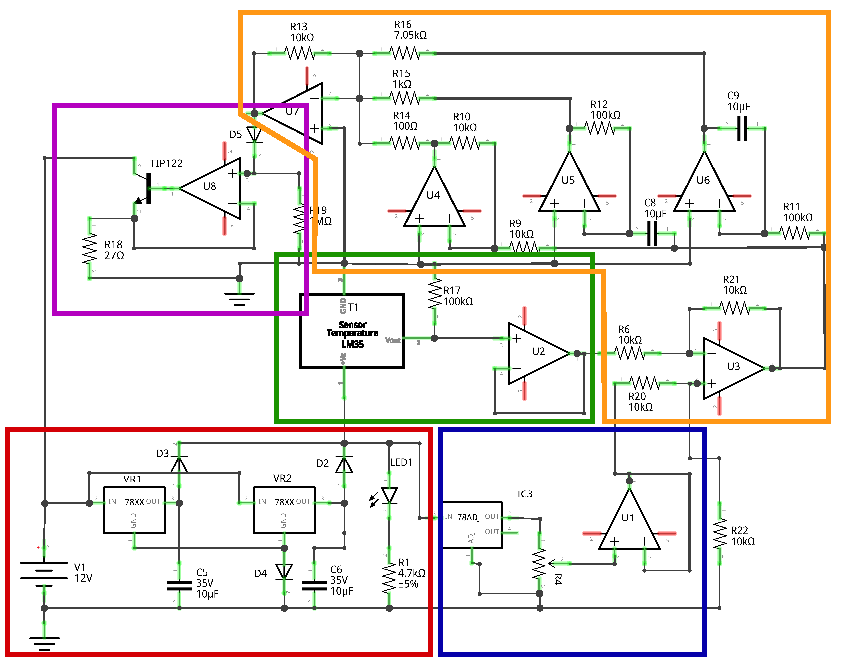
\includegraphics[width=0.9\linewidth]{extras/circuit_schem.pdf}
	\caption{Circuito PID, implementado para el control de la temperatura.}
	\label{fig: circuito}
\end{figure}

\section{Calibraci\'on de la temperatura}
El sensor de temperatura corresponde con un LM35, circuito integrado con respuesta lineal a la temperatura, con un factor de escala de 10 mV/$^\circ$C y un rango de operaci\'on de -55 $^\circ$C a 150 $^\circ$C \cite{LM35}. A pesar de ser un sensor calibrado, se realiza una calibraci\'on \textit{in situ} usando una termocupla de NiCr-Ni Phywe.
\begin{figure}[h]
	\centering
	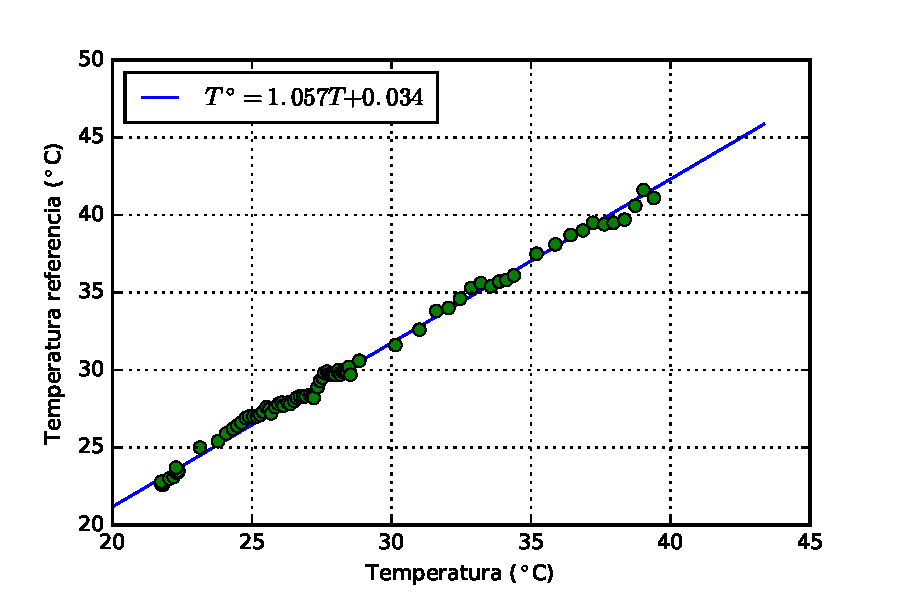
\includegraphics[width=0.6\linewidth]{extras/temp_cal.pdf}
	\caption{Calibraci\'on del sensor.}
	\label{fig: temp calibration}
\end{figure}

Los resultados se muestran en la Figura \ref{fig: temp calibration}, de donde se observa la linealidad del sensor usado, tanto la pendiente como el intercepto muestran desfases del valor esperado (1 y 0, correspondientemente) sobre la seg\'unda cifra decimal, discrepancias menores al 6 \%.

\section{Caracterizaci\'on del actuador}
Inicialmente la construcci\'on del horno usaba una celda Peltier, no obstante esta dej\'o de funcionar. Por este motivo se modifica el actuador a una resistencia de 27 $\Omega$ y 5 vatios. Para una resistencia la potencia es proporcional al cuadrado de la diferencia de potencial entre sus terminales:
\begin{equation}
	P = VI = V\left(\frac{V}{R}\right)
\end{equation}

\begin{figure}[h]
	\centering
	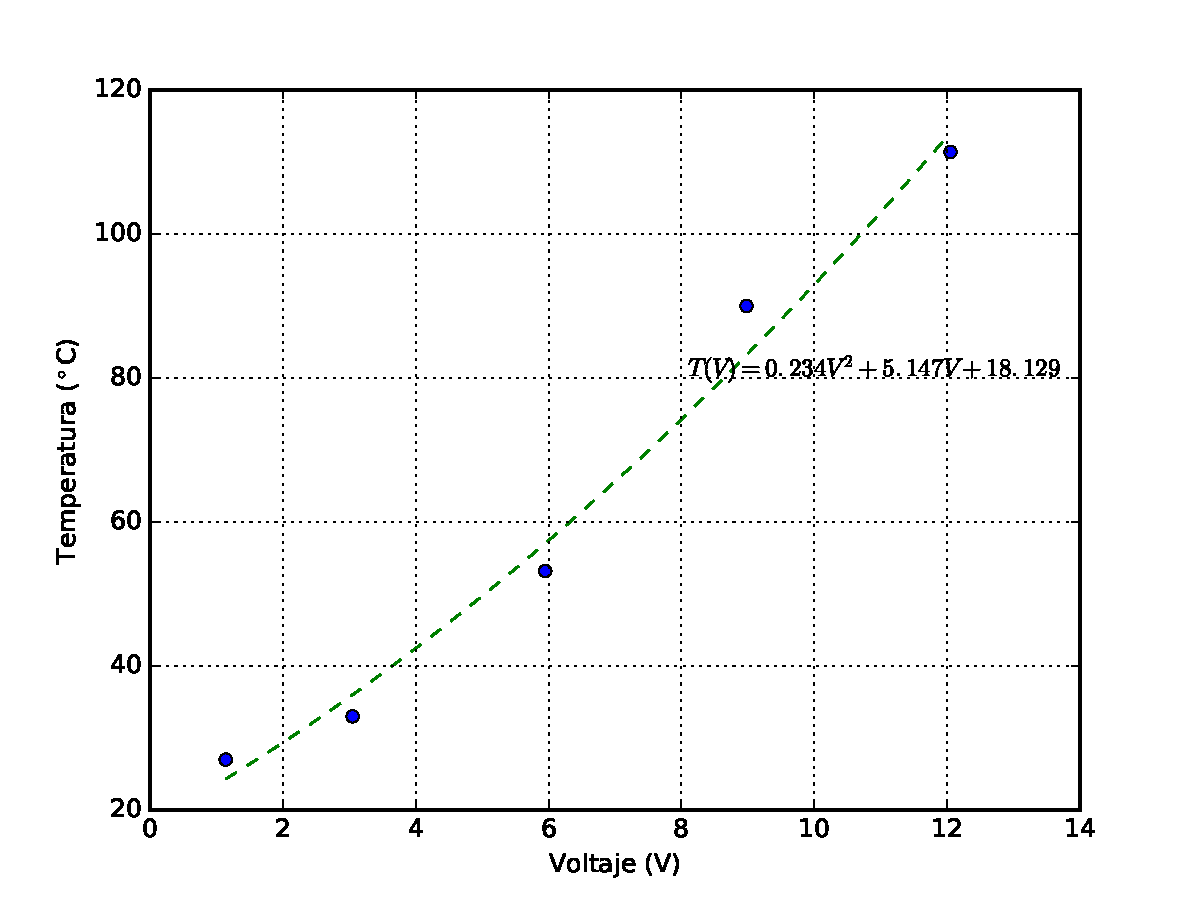
\includegraphics[width=0.6\linewidth]{extras/actuator.pdf}
	\caption{Temperaturas alcanzadas por la resistencia para distintos valores de voltaje.}
\end{figure}
Debido a que el sistema se encuentra restringido a voltajes de $\pm$12 y 0 V, la m\'axima potencia sobre la resistencia ser\'a 5.3 W, valor que se encuentra dentro de la capacidad de la resistencia.

\section{Sistema de alimentaci\'on}
El sistema de alimentaci\'on est\'a compuesto por dos reguladores de voltaje de 5 V de la familia 7805 \cite{7805}. El circuito de alimentaci\'on se encuentra acompa\~nado de dos condensadores que act\'uan como filtros, adem\'as se dispone de tres diodos 1N4001 \cite{1N4001} como protecci\'on a corriente reversa. El circuito sin carga mantiene un potencial de 5.03 V, y con carga se alcanzan valores de 4.78 V.
\begin{figure}[h]
	\centering
	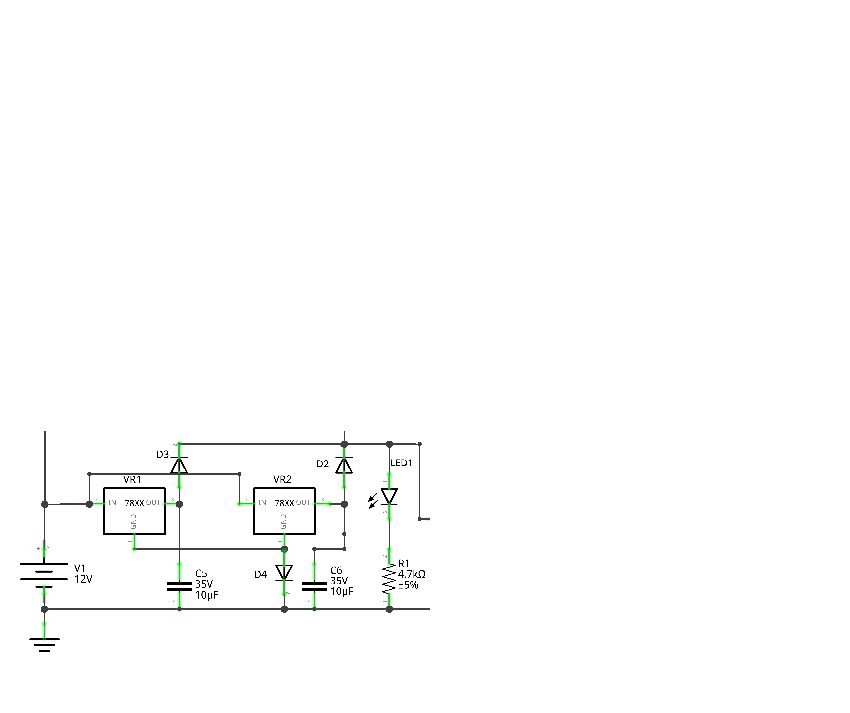
\includegraphics[width=0.9\linewidth]{extras/alimentacion.pdf}
	\caption{Circuito de alimentaci\'on del horno.}
\end{figure}

\section{Controlador}
El controlador est\'a compuesto por tres etapas:
\begin{itemize}
	\item \textbf{Restador:} calcula el error en la temperatura del horno.
	\item \textbf{PID:} todas las partes invierten la salida y mantienen la ganancia en 1.
	\item \textbf{Sumador:} se suma de forma ponderada las distintas componentes del PID. Las constantes usadas se muestran en la Tabla \ref{tb: PID}.
	
	\begin{table}[h]
		\centering
		\caption{Par\'ametros del controlador PID.}
		\begin{tabular}{|c|c|}
			\hline
			$K_P$ & 100 \\
			$K_I$ & 10 \\
			$K_D$ & 1.42 \\
			\hline
		\end{tabular}
		\label{tb: PID}
	\end{table}
\end{itemize}

Los par\'ametros del controlador fueron determinados manualmente. En primer lugar se determin\'o $K_P$ usando 8 valores distintos de $R_{13}$.
\begin{equation}
	K_P = \frac{R_{14}}{R_{13}}
\end{equation}

\begin{figure}[h]
	\centering
	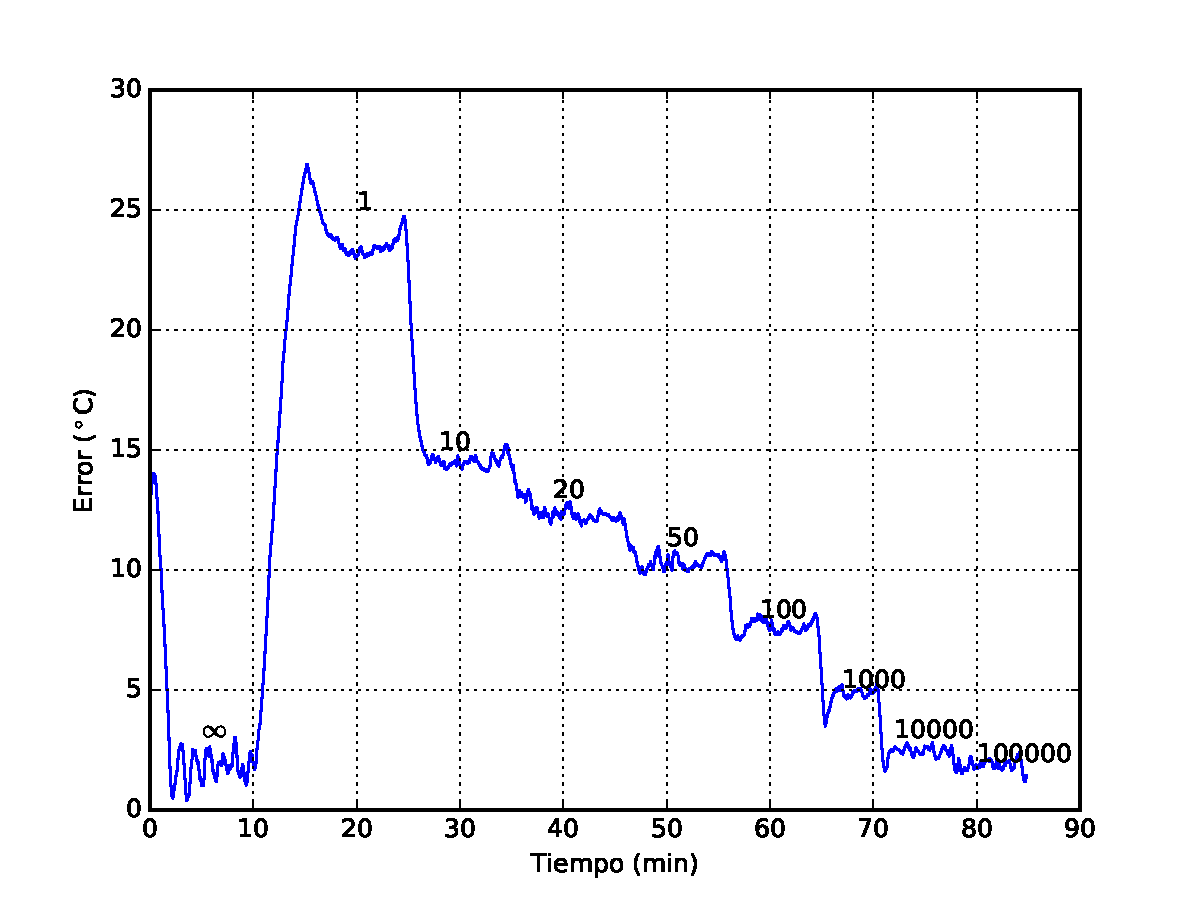
\includegraphics[width=0.6\linewidth]{extras/KP.pdf}
\end{figure}
En segundo lugar se agrega la etapa derivativa, para la cual la ganancia $K_D$ corresponde con;
\begin{equation}
	K_D = \frac{R_{14}}{R_{15}}
\end{equation}

\begin{figure}[h]
	\centering
	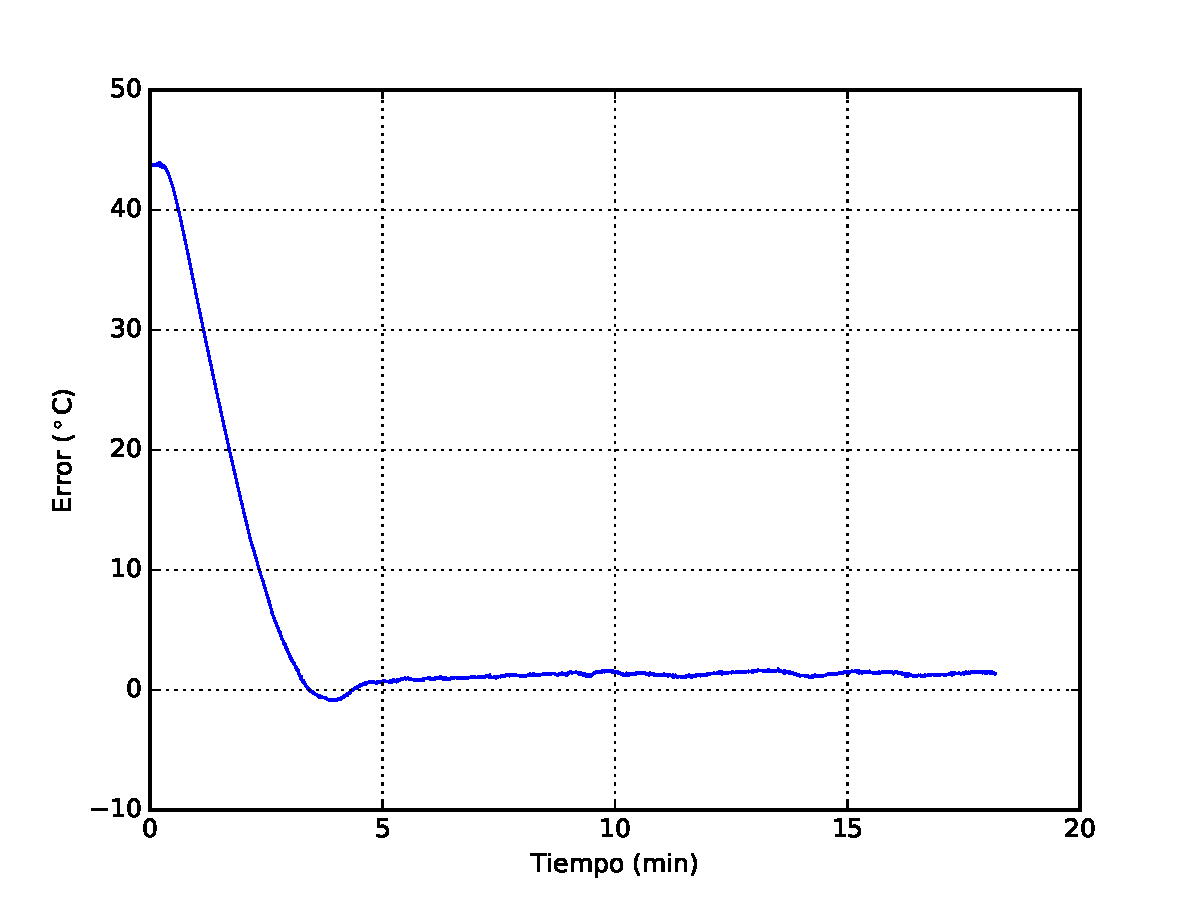
\includegraphics[width=0.6\linewidth]{extras/final_PID.pdf}
	\caption{Resultado final del controlador PID.}
\end{figure}
Finalmente se agrega una etapa integradora para eliminar el error del estado estacionario, los valores de $K_I$ con los que se prob\'o el circuito fueron: 10, 1 y 1.42. El primero, satura permanentemente el actuador, manteniendo siempre al m\'aximo la diferencia de potencial. Con el segundo se alcanza un error del estado estacionario para una temperatura de 67.6 $^\circ$C en 3 $^\circ$C, error que se reduce con la \'ultima constante a cerca de 1 $^\circ$C.

\section{Digitalizaci\'on}
El valor de referencia es fijado usando un potenciometro digital con referencia X9C103P \cite{digi-pot} con resistencia interna de 100 k$\Omega$. Los tres pines l\'ogicos son conectados a los GPIO, los puertos predeterminados son:
\begin{enumerate}
	\item[19] \textbf{IN} (INCREMENT) 
	\item[20] \textbf{U/D} (UP/DOWN)
	\item[21] \textbf{C/S} (CHIP SELECT)
\end{enumerate}

Sin embargo los mismos pueden ser modificados usando la interf\'az gr\'afica. A continuaci\'on se muestran dos curvas del potencial en funci\'on de la posici\'on de la aguja del potenci\'ometro.
\begin{figure}[h]
	\begin{tabular}{cc}
		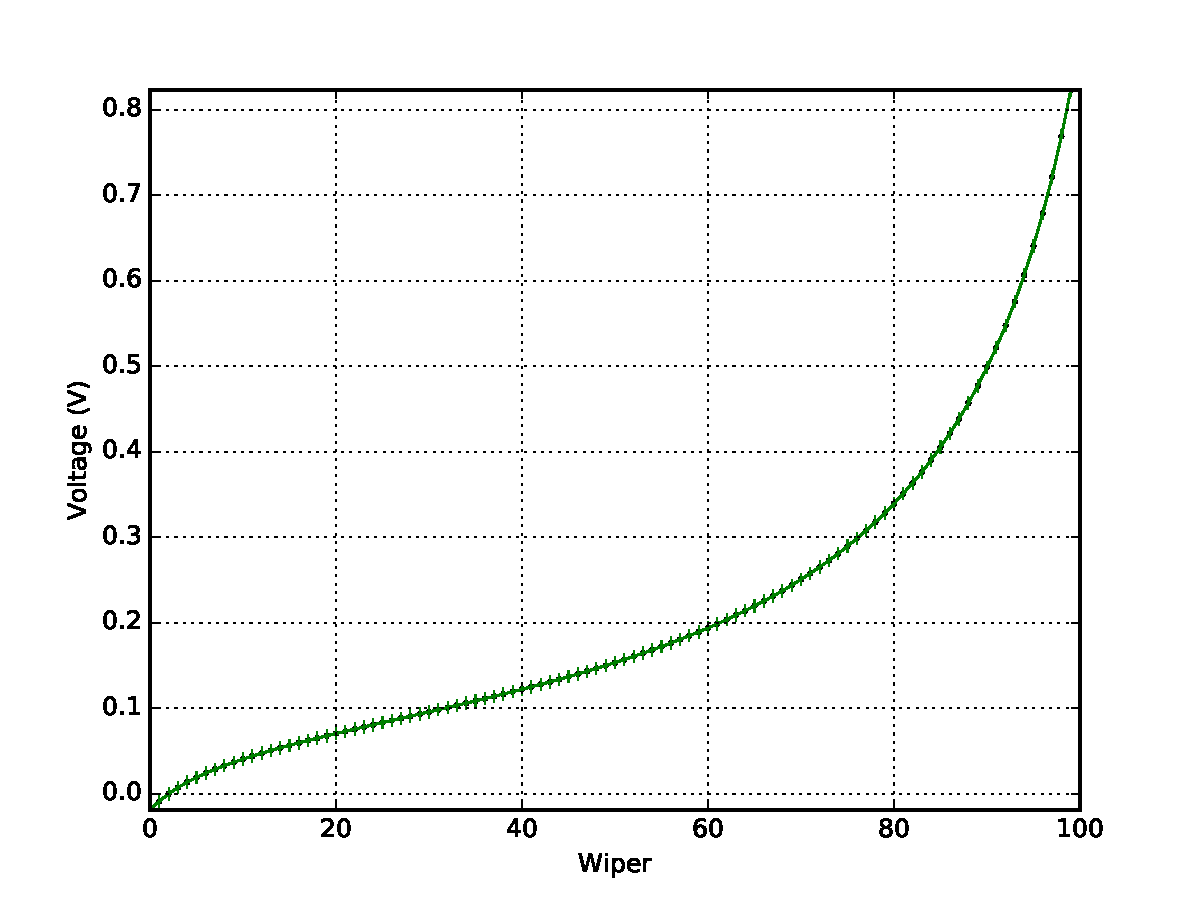
\includegraphics[width=0.5\linewidth]{extras/without_follower.pdf}
		& 
		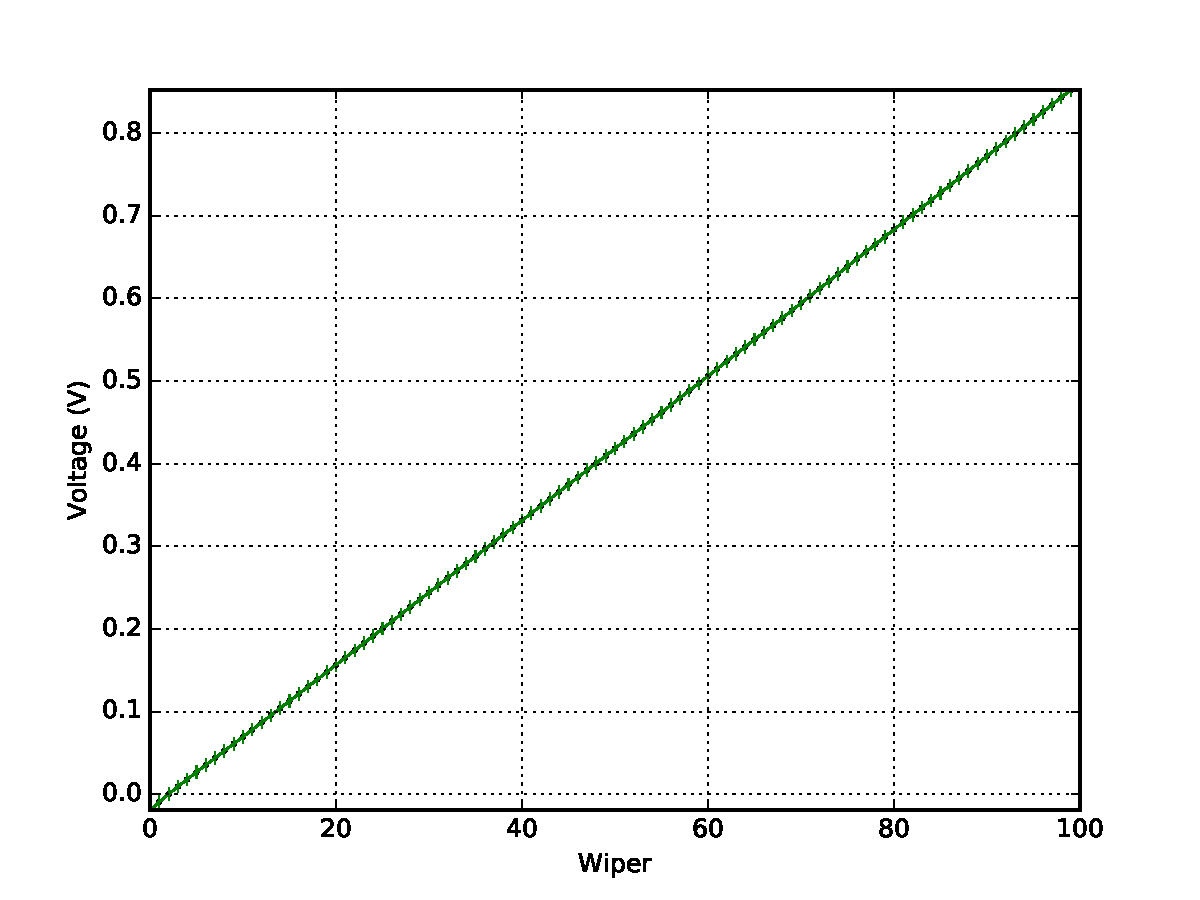
\includegraphics[width=0.5\linewidth]{extras/with_follower.pdf}
	\end{tabular}
	\caption{Voltaje de salida del potenci\'ometro acoplado al restador del PID. A la izquierda con carga, en el derecho con seguidor.}
\end{figure}

En las figuras anteriores se puede apreciar el efecto de la carga sobre el divisor de voltaje. Una modificaci\'on final en la etapa de digitalizaci\'on permiti\'o lograr un rango de potenciales de 0 a 3.3 V, conservando la linealidad, pero reduciendo la selecci\'on de temperaturas a cada 3.3 $^\circ$C.

\begin{figure}[h]
	\centering
	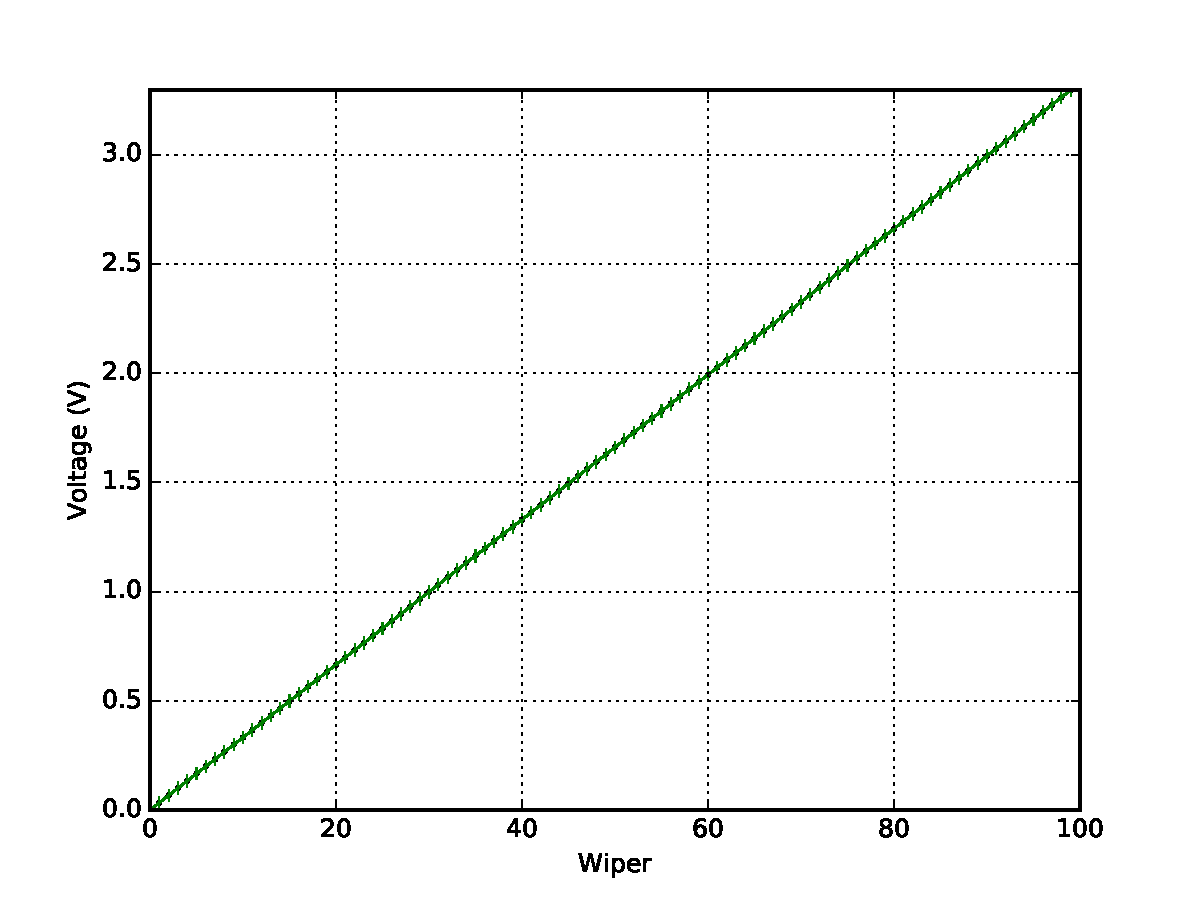
\includegraphics[width=0.4\linewidth]{extras/final_cal.pdf}
	\caption{Calibraci\'on final del potenciometro digital.}
\end{figure}
\begin{chapreferences}{10.}
	\bibitem{LM35} Texas Instruments, ``LM35 Precision	Centigrade Temperature Sensors'' LM35 datasheet, Aug. 1999 [Revised Aug.
	2016].
	\bibitem{7805} Spark fun ``Positive-Voltage Regulators'' $\mu$A7805C datasheet, May. 1976 [Revised May. 2003].
	\bibitem{1N4001} Diodes, ``Diffused Junction 1N4001 - 1N4007'' 1N4001 datasheet, Sep. 2004.
	\bibitem{digi-pot}
	Digitally Controlled Potentiometer ``X9C103'' datasheet, Jul 2009.
\end{chapreferences}

\chapter{Algoritmo}

%%%%%%%%%%%%%%%%%%%%%%%%%%%%%%%%%%%%%%%%%%%%%%%%%%%%%%
%% optional prologue or prologues
% \chapter{Chapter Title}
% \prologue{<text>}{<author attribution>}

%%%%%%%%%%%%%%%%%%%%%%%%%%%%%%%%%%%%%%%%%%%%%
% Edited Book: Author and Affiliation
%%%%%%%%%%%%%%%%%%%%%%%%%%%%%%%%%%%%%%%%%%%%%

% After \chapter{Chapter Title}, you can
% enter the author name and embed the affiliation with
% \chapterauthors{(author name, or names)
% \chapteraffil{(affiliation or affiliations)}
% }    

% For instance:
% \chapter{Chapter Title}
% \chapterauthors{G. Alvarez and R. K. Watts
% \chapteraffil{Carnegie Mellon University, Pittsburgh, Pennsylvania}

% For separate affiliations you can use \affilmark{(number)} after
% the name of a particular author and before the matching affiliation:

% For instance:
% \chapter{Chapter Title}
% \chapterauthors{George Smeal, Ph.D.\affilmark{1}, Sally Smith,
% M.D.\affilmark{2}, and Stanley Kubrick\affilmark{1}
% \chapteraffil{\affilmark{1}AT\&T Bell Laboratories
% Murray Hill, New Jersey\\
% \affilmark{2}Harvard Medical School,
% Boston, Massachusetts}
% }

%%%%%%%%%%%%%%%%%%%%%%%

%% short version of section head, or one without \\ supplied in sq. brackets.

% \section[Introduction and fugue]{Introduction\\ and fugue}
% \subsection[This is the subsection]{This is the\\ subsection}
% \subsubsection{This is the subsubsection}
% \paragraph{This is the paragraph}

% \begin{chapreferences}{widest label}
% \bibitem{<label>}Reference
% \end{chapreferences}

% optional chapter bibliography using BibTeX,
% must also have \usepackage{chapterbib} before \begin{document}
% Must use root file with \include{chap1}, \include{chap2} form.
%\bibliographystyle{plain}
%\bibliography{<your .bib file name>}

% optional appendix at the end of a chapter:
% \chapappendix{<chap appendix title>}
% \chapappendix{} % no title

%%%%%%%%%%%%%%%%%%%%%%%%%%%%%%%%%%%%%%%%%%%%%%%%%%%%%%%%%%%%%%%%
%% End Matter >>>>>>>>>>>>>>>>>>

% \appendix{<optional title for appendix at end of book>}
% \appendix{} % appendix without title

% \begin{references}{<widest label>}
% \bibitem{sampref}Here is reference.
% \end{references}

%%%%%%%%%%%%%%%%%%%%%%%%%%%%%%%%%%%%%%%%%%%%%%%%%%%%%%%%%%%%%%%%
%% Optional Problem Sets: Can use this at the end of each chapter or at end
%% of book

% \begin{problems}
% \prob
% text

% \prob
% text

% \subprob
% text

% \subprob
% text

% \prob
% text
% \end{problems}

%%%%%%%%%%%%%%%%%%%%%%%%%%%%%%%%%%%%%%%%%%%%%%%%%%%%%%%%%%%%%%%%
%% Optional Exercises: Can use this at the end of each chapter or at end
%% of book

% \begin{exercises}
% \exer
% text

% \exer
% text

% \subexer
% text

% \subexer
% text

% \exer
% text
% \end{exercises}


%%%%%%%%%%%%%%%%%%%%%%%%%%%%%%%%%%%%%%%%%%%%%%%%%%%%%%%%%%%%%%%%
%% INDEX: Use only one index command set:

%% 1) The default LaTeX Index
\printindex

%% 2) For Topic index and Author index:

% \usepackage{multind}
% \makeindex{topic}
% \makeindex{authors}
% \begin{document}
% ...
% add index terms to your book, ie,
% \index{topic}{A term to go to the topic index}
% \index{authors}{Put this author in the author index}

%% (these are Wiley commands)
%\multiprintindex{topic}{Topic index}
%\multiprintindex{authors}{Author index}

\end{document}

%%%%%%% Demo of section head containing sample macro:
%% To get a macro to expand correctly in a section head, with upper and
%% lower case math, put the definition and set the box 
%% before \begin{document}, so that when it appears in the 
%% table of contents it will also work:

\newcommand{\VT}[1]{\ensuremath{{V_{T#1}}}}

%% use a box to expand the macro before we put it into the section head:

\newbox\sectsavebox
\setbox\sectsavebox=\hbox{\boldmath\VT{xyz}}

%%%%%%%%%%%%%%%%% End Demo


Other commands, and notes on usage:

-----
Possible section head levels:
\section{Introduction}
\subsection{This is subsection}
\subsubsection{This is subsubsection}
\paragraph{This is the paragraph}

-----
Tables:
 Remember to use \centering for a small table and to start the table
 with \hline, use \hline underneath the column headers and at the end of 
 the table, i.e.,

\begin{table}[h]
\caption{Small Table}
\centering
\begin{tabular}{ccc}
\hline
one&two&three\\
\hline
C&D&E\\
\hline
\end{tabular}
\end{table}

For a table that expands to the width of the page, write

\begin{table}
\begin{tabular*}{\textwidth}{@{\extracolsep{\fill}}lcc}
\hline
....
\end{tabular*}
%% Sample table notes:
\begin{tablenotes}
$^a$Refs.~19 and 20.

$^b\kappa, \lambda>1$.
\end{tablenotes}
\end{table}

-----
Algorithm.
Maintains same fonts as text (as opposed to verbatim which uses fixed
width fonts). Space at beginning of line will be maintained if you
use \ at beginning of line.

\begin{algorithm}
{\bf state\_transition algorithm} $\{$
\        for each neuron $j\in\{0,1,\ldots,M-1\}$
\        $\{$   
\            calculate the weighted sum $S_j$ using Eq. (6);
\            if ($S_j>t_j$)
\                    $\{$turn ON neuron; $Y_1=+1\}$   
\            else if ($S_j<t_j$)
\                    $\{$turn OFF neuron; $Y_1=-1\}$   
\            else
\                    $\{$no change in neuron state; $y_j$ remains %
unchanged;$\}$ .
\        $\}$   
$\}$   
\end{algorithm}

-----
Sample quote:
\begin{quote}
quotation...
\end{quote}

-----
Listing samples

\begin{enumerate}
\item
This is the first item in the numbered list.

\item
This is the second item in the numbered list.
\end{enumerate}

\begin{itemize}
\item
This is the first item in the itemized list.

\item
This is the first item in the itemized list.
This is the first item in the itemized list.
This is the first item in the itemized list.
\end{itemize}

\begin{itemize}
\item[]
This is the first item in the itemized list.

\item[]
This is the first item in the itemized list.
This is the first item in the itemized list.
This is the first item in the itemized list.
\end{itemize}

%% Index commands
Author and Topic Indices, See docs.pdf and w-bksamp.pdf
